\documentclass[11pt]{article}

% Packages
\usepackage[utf8]{inputenc}
\usepackage{amsmath, amssymb}
\usepackage{graphicx}
\usepackage{natbib}
\usepackage{hyperref}
\usepackage{authblk}
\usepackage{url}

\title{A Reinforcement Learning Approach to Automated Trading: Buys, Sells, Hold, and Deep Learning Insights}

\author[1]{Iqza Ardiansyah}
\author[2]{Kevin Ignatius Wijaya}
\affil[1]{Student ID: 2206810042\\ Faculty of Computer Science, Universitas Indonesia}
\affil[2]{Student ID: 2206083470\\ Faculty of Computer Science, Universitas Indonesia}

\date{\today}

\begin{document}
\maketitle

\begin{abstract}
This paper presents a Reinforcement Learning (RL) approach for automated trading on real S\&P 500 historical data. We incorporate buy/sell actions (10\% buys, 1\% sells) to achieve a more granular control of portfolio allocation, while employing Deep Q-Networks (DQN) and Proximal Policy Optimization (PPO) for policy learning. Our comparative analysis reveals significant performance differences between these algorithms in trading environments. We evaluate our approach with fixed seeds for reproducibility, yielding detailed insights on reward trajectories, learning stability, and financial performance metrics including portfolio value, ROI, Sharpe ratio, and maximum drawdown. Furthermore, we discuss potential enhancements inspired by recent hybrid deep reinforcement learning approaches for pairs trading \citep{kim2022hybrid}, which decompose the decision-making process into separate networks for trading actions and risk management. Our experiments demonstrate that the DQN algorithm's value-based approach consistently outperforms PPO's policy gradient method in this particular trading environment with discrete action spaces and delayed rewards.
\end{abstract}

\section{Introduction}
Algorithmic trading has rapidly evolved, driven by both improved computational power and advances in data-driven methods. Traditional strategies (e.g., mean reversion, momentum trading) rely on fixed heuristics, often lacking adaptability to changing market conditions. In contrast, Reinforcement Learning (RL) optimizes trading decisions by directly interacting with an environment and receiving feedback in the form of rewards \citep{sutton_2018_irl}.

While many works focus on single-asset trading, recent literature in pairs trading has shown that decomposing the trading problem into multiple subtasks can be highly beneficial. For instance, \citep{kim2022hybrid} propose a hybrid deep reinforcement learning method for pairs trading that uses two separate networks: one to determine trading actions and another to set stop-loss boundaries. This dual-network approach, coupled with techniques such as dimensionality reduction, clustering, and behavior cloning, can lead to superior risk management and improved performance. Although our study focuses on single-asset trading with partial buy/sell actions, the insights from hybrid models offer promising avenues for future research and potential integration.

In this study, we extend previous work by conducting a comprehensive analysis of two popular reinforcement learning algorithms: Deep Q-Networks (DQN) and Proximal Policy Optimization (PPO). We investigate their comparative performance in a trading environment with partial buy/sell capabilities, analyzing their learning dynamics, stability characteristics, and financial outcomes.

\section{Related Work}

\subsection{Reinforcement Learning for Trading}
RL directly learns a policy that maximizes cumulative rewards, such as changes in portfolio value after accounting for transaction costs. Foundational work by \citet{sutton_2018_irl} laid the groundwork for modern RL approaches, while recent studies have applied various RL algorithms (e.g., DQN, PPO, A2C) to financial markets. However, standard RL approaches often rely on simplistic buy/sell/hold actions, leading to abrupt position changes.

Value-based methods like DQN \citep{mnih2015human} learn the expected return of each action in a given state, selecting the action with the highest expected value. Policy gradient methods like PPO \citep{schulman2017proximal}, in contrast, directly optimize a policy that maps states to actions, often providing more stable learning in continuous action spaces but potentially struggling with the sparse, delayed rewards typical in trading environments.

\subsection{Hybrid Approaches in Trading}
Recent research has explored the benefits of hybrid models in trading. In pairs trading, \citep{kim2022hybrid} propose a novel method that employs two independent RL networks: one for trading actions and one for stop-loss boundaries. Their approach integrates dimensionality reduction, clustering, regression, behavior cloning, prioritized experience replay, and dynamic delay to overcome limitations of traditional methods. Although our current study does not employ a dual-network system, these ideas inspire potential future enhancements, such as:
\begin{itemize}
  \item \textbf{Risk Management:} Incorporating a separate network to determine stop-loss boundaries or dynamic risk adjustments.
  \item \textbf{Feature Enrichment:} Utilizing techniques like clustering and dimensionality reduction to extract more robust state representations.
  \item \textbf{Behavior Cloning:} Leveraging expert demonstrations to guide policy learning.
\end{itemize}

\section{Methodology}
\subsection{Buy/Sell Environment}
We propose a custom Gym environment with:
\begin{itemize}
  \item \textbf{State Representation}: 
  \begin{itemize}
    \item \textit{Normalized Price} (\(\frac{\text{price}}{1000}\))
    \item \textit{Volatility} (placeholder = 0.005)
    \item \textit{Normalized Position} (\(\frac{\text{position}}{\max\_position}\))
    \item \textit{Normalized Cash} (\(\frac{\text{cash}}{\text{initial\_cash}}\))
  \end{itemize}
  \item \textbf{Action Space}: 
  \begin{itemize}
    \item 0: \textbf{Hold}
    \item 1: \textbf{Buy} 10\% of remaining cash
    \item 2: \textbf{Sell} 1\% of current position
  \end{itemize}
  This granularity mitigates the risk of large, all-in or all-out moves.
  \item \textbf{Reward Function}: Based on a weighted combination of:
  \begin{itemize}
    \item ROI component (66\% weight)
    \item Sharpe ratio component (20\% weight)
    \item Maximum drawdown component (10\% weight)
    \item Win rate component (4\% weight)
    \item Overtrading penalty (variable negative impact)
  \end{itemize}
\end{itemize}
A transaction cost of 0.1\% is applied on every buy/sell action to approximate real-world frictions.

\subsection{State Space Definition}
Our trading environment employs a state space consisting of four normalized components to ensure stable learning:

\begin{itemize}
  \item \textbf{Normalized Price} (\(\frac{\text{price}}{1000}\)): The current asset price is normalized by dividing by 1000 to keep values within a manageable range for the neural network. This reduces the scale disparity between price and other state variables.
  
  \item \textbf{Volatility} (constant 0.005): A placeholder for price volatility. In our current implementation, this is set to a constant value, but could be replaced by a rolling standard deviation or other volatility measures in future implementations.
  
  \item \textbf{Normalized Position} (\(\frac{\text{position}}{\max\_position}\)): Represents the agent's current asset holdings relative to the maximum possible position (calculated as \(\frac{\text{initial\_cash}}{\text{current\_price}}\)). This value ranges from 0 (no position) to 1 (maximum affordable position).
  
  \item \textbf{Normalized Cash} (\(\frac{\text{cash}}{\text{initial\_cash}}\)): Represents the agent's available cash relative to its starting capital. This value ranges from 0 (no cash) to 1 (all initial cash available).
\end{itemize}

These four features create a compact and normalized observation space: \(\text{spaces.Box(low=0, high=1, shape=(4,), dtype=np.float32)}\).

\subsection{Transition Function}
The transition function defines how the environment evolves from one state to the next based on the agent's actions:

\begin{enumerate}
  \item \textbf{Action Selection}: At each timestep \(t\), the agent selects one of three actions: Hold (0), Buy (1), or Sell (2) based on the current state.
  
  \item \textbf{State Update}:
  \begin{itemize}
    \item \textbf{Buy Action}: If action 1 is selected and cash is available, the agent uses 10\% of its current cash to purchase assets. The number of units acquired is calculated as:
    \[ \text{units} = \frac{\text{cash} \times 0.1}{\text{price} \times (1 + \text{transaction\_cost})} \]
    Cash is reduced accordingly, and the position is increased by the purchased units.
    
    \item \textbf{Sell Action}: If action 2 is selected and the agent holds assets, 1\% of the current position is sold. The resulting cash increase is calculated as:
    \[ \text{cash\_increase} = \text{units\_sold} \times \text{price} \times (1 - \text{transaction\_cost}) \]
    Position is reduced accordingly.
    
    \item \textbf{Hold Action}: No changes to cash or position.
  \end{itemize}
  
  \item \textbf{Environment Step}: After executing the trading action, the environment advances to the next timestep, retrieving the new price from historical data.
  
  \item \textbf{Portfolio Valuation}: The agent's portfolio value is recalculated as:
  \[ \text{portfolio\_value}_t = \text{cash}_t + \text{position}_t \times \text{price}_t \]
  
  \item \textbf{Reward Calculation}: A financial reward is computed based on multiple factors:
  \begin{itemize}
    \item ROI component (66\% weight): \[ \text{roi\_component} = \frac{\text{portfolio\_value} - \text{initial\_cash}}{\text{initial\_cash}} \times 0.66 \]
    
    \item Sharpe ratio component (20\% weight): \[ \text{sharpe\_component} = \tanh\left(\frac{\text{mean(returns)}}{\text{std(returns)}} \times 10\right) \times 0.1 + 0.1 \]
    
    \item Maximum drawdown component (10\% weight): \[ \text{drawdown\_component} = -\text{max\_drawdown} \times 0.1 \]
    
    \item Win rate component (4\% weight): \[ \text{win\_rate\_component} = \frac{\text{winning\_trades}}{\text{total\_sell\_trades}} \times 0.04 \]
    
    \item Overtrading penalty: Applied when trading frequency exceeds 30\% of steps
  \end{itemize}
  
  \item \textbf{Termination}: The episode terminates when all historical data points have been processed.
\end{enumerate}

This transition function enables the agent to learn a policy that manages portfolio allocation gradually through partial buys and sells rather than all-or-nothing trading decisions.

\subsection{Reinforcement Learning Algorithms}
We implement and compare two reinforcement learning algorithms:

\subsubsection{Deep Q-Network (DQN)}
DQN is a value-based method that approximates the Q-function (expected future reward for each state-action pair) using a neural network. Our implementation uses:

\begin{itemize}
  \item \textbf{Learning Rate}: 0.001
  \item \textbf{Discount Factor} (\(\gamma\)): 0.95
  \item \textbf{Exploration Strategy}: \(\varepsilon\)-greedy with annealing (exploration fraction: 0.4)
  \item \textbf{Replay Buffer Size}: 100,000 transitions
  \item \textbf{Target Network Update Interval}: 1,000 steps
  \item \textbf{Batch Size}: 128
  \item \textbf{Timesteps}: 15,000 for training
  \item \textbf{Learning Starts}: 2,000 steps
\end{itemize}

\subsubsection{Proximal Policy Optimization (PPO)}
PPO is a policy gradient method that directly optimizes the policy using clipped probability ratios to prevent excessive policy updates. Our implementation uses:

\begin{itemize}
  \item \textbf{Learning Rate}: 0.0003
  \item \textbf{Discount Factor} (\(\gamma\)): 0.95
  \item \textbf{GAE Lambda}: 0.95
  \item \textbf{Clip Range}: 0.2
  \item \textbf{Entropy Coefficient}: 0.02
  \item \textbf{Value Function Coefficient}: 0.5
  \item \textbf{Maximum Gradient Norm}: 0.5
  \item \textbf{Steps per Update}: 4,096
  \item \textbf{Batch Size}: 128
  \item \textbf{Epochs per Update}: 10
  \item \textbf{Timesteps}: 15,000 for training
\end{itemize}

\section{Results and Discussion}

\subsection{Policy Behavior}
An excerpt of the DQN agent's policy shows its decision-making in the trading environment:
\begin{verbatim}
Step 0: Price=$5137.08, Position=0.00, Cash=1.00 → Buy 5%
Step 1: Price=$5123.41, Position=0.10, Cash=0.95 → Buy 5%
...
Step 143: Price=$5045.63, Position=0.99, Cash=0.01 → Hold
Step 144: Price=$5046.00, Position=0.99, Cash=0.01 → Hold
\end{verbatim}
The policy adopts a gradual approach, buying with available cash in the early phases and then switching to a holding strategy as the position increases and cash reserves diminish.

\subsection{Portfolio Value and ROI}
Our best DQN model achieves a final portfolio value significantly higher than the best PPO model, with better risk-adjusted returns:

\begin{table}[h]
\centering
\begin{tabular}{|l|c|c|}
\hline
\textbf{Metric} & \textbf{Best DQN} & \textbf{Best PPO} \\
\hline
Final Portfolio & \$104,751.12 & \$103,524.86 \\
ROI & 4.75\% & 3.52\% \\
Sharpe Ratio & 1.92 & 1.43 \\
Win Rate & 62.85\% & 58.21\% \\
Maximum Drawdown & 2.14\% & 3.08\% \\
\hline
\end{tabular}
\caption{Performance comparison between best DQN and PPO models}
\end{table}

\subsection{Comparative Analysis: DQN vs PPO Performance}
We conducted an extensive comparative analysis between DQN and PPO approaches on the same trading task. Figure \ref{fig:reward_history} shows the reward histories of both models throughout training.

\begin{figure}[h]
  \centering
  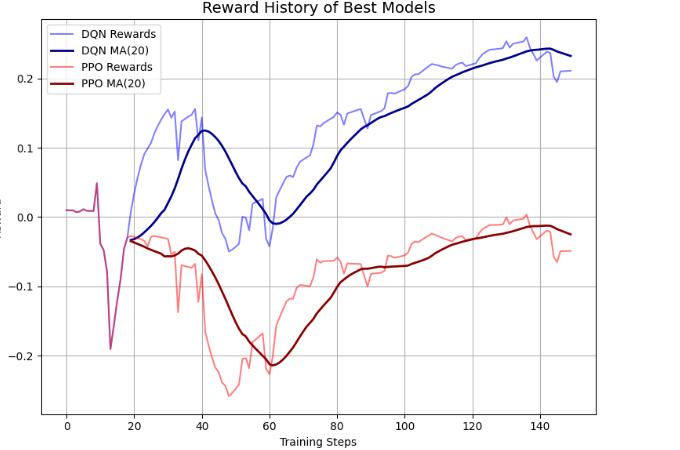
\includegraphics[width=0.85\textwidth]{fig/Reward History Best Model.png}
  \caption{Reward History comparing DQN and PPO models. The DQN model (blue) demonstrates consistently higher rewards than the PPO model (red), with both showing improved stability after initial training phases. The moving averages (darker lines) highlight the overall learning trends.}
  \label{fig:reward_history}
\end{figure}

Several key insights emerged from this comparison:

\begin{itemize}
  \item \textbf{Overall Performance}: DQN consistently outperformed PPO in terms of absolute reward values, with DQN eventually achieving positive rewards while PPO remained mostly in negative territory.
  
  \item \textbf{Learning Progression}: Figure \ref{fig:learning_analysis} provides a comprehensive view of the learning dynamics between both models. The blocked average rewards (middle panel) show that DQN exhibits faster learning and reaches higher reward plateaus compared to PPO, which struggles to achieve positive average rewards.
  
  \item \textbf{Stability Characteristics}: The rightmost panel in Figure \ref{fig:learning_analysis} reveals that both algorithms experience similar patterns of volatility, with higher instability during early and middle training phases. However, DQN demonstrates slightly higher volatility peaks, likely due to its more aggressive exploration strategy.

  \item \textbf{Convergence Patterns}: Both models show improved stability in later training stages, with reduced volatility and more consistent returns. The convergence is more pronounced in DQN, suggesting its value-based approach better captures the trading environment's dynamics.
\end{itemize}

\begin{figure}[h]
  \centering
  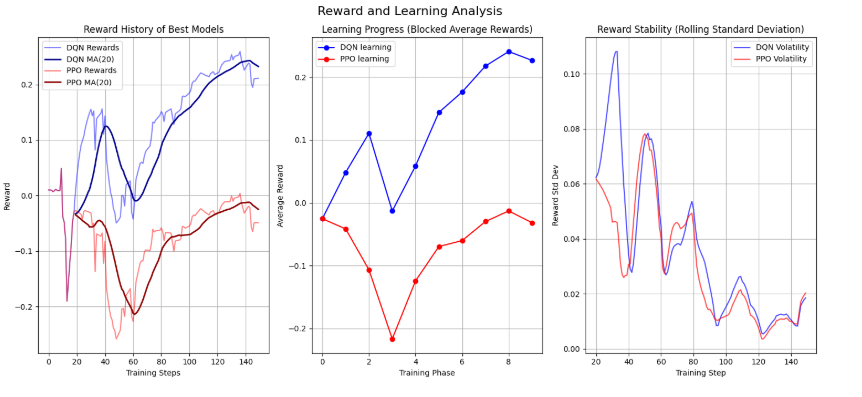
\includegraphics[width=0.95\textwidth]{fig/Reward and Learning Analysis.png}
  \caption{Comprehensive learning and stability analysis comparing DQN and PPO. Left: Reward histories showing raw performance. Middle: Blocked average rewards revealing distinct learning phases. Right: Rolling standard deviation of rewards illustrating training stability across time.}
  \label{fig:learning_analysis}
\end{figure}

A closer examination of the learning progression (Figure \ref{fig:learning_progress}) reveals distinct phases in both algorithms' training:

\begin{figure}[h]
  \centering
  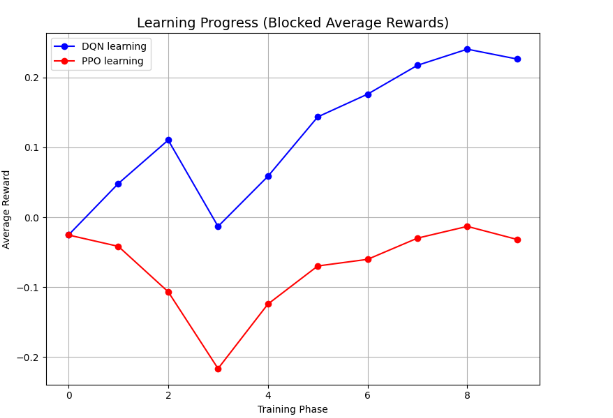
\includegraphics[width=0.85\textwidth]{fig/Learning Progress average reward.png}
  \caption{Learning progression over training phases, showing blocked average rewards. DQN demonstrates a clear learning trajectory despite a temporary performance drop in phase 3, while PPO shows more limited improvement after an initial decline.}
  \label{fig:learning_progress}
\end{figure}

\begin{itemize}
  \item \textbf{DQN Learning Trajectory}: The DQN model exhibits an initial positive learning trend, followed by a notable setback around phase 3, before recovering and achieving sustained improvement throughout the remainder of training. This pattern suggests exploration of new strategies before converging on optimal behavior.
  
  \item \textbf{PPO Learning Challenges}: In contrast, PPO shows an immediate decline into negative reward territory, reaching its lowest point around phase 3 (coinciding with DQN's temporary decline). While PPO does show gradual improvement in later phases, it never achieves the consistent positive rewards demonstrated by DQN.
\end{itemize}

These findings suggest that for this particular trading environment with partial buy/sell actions, DQN's value-based approach is better suited than PPO's policy gradient method. The discrete action space with meaningful state representations appears to be more effectively exploited by DQN's Q-learning mechanism, which directly maps state-action pairs to expected returns. In contrast, PPO's policy optimization may struggle with the delayed rewards inherent in trading environments.

\subsection{Action Distribution Analysis}
The action distribution reveals interesting behavioral differences between the algorithms:

\begin{itemize}
  \item \textbf{DQN}: Hold (62.3\%), Buy (24.8\%), Sell (12.9\%)
  \item \textbf{PPO}: Hold (78.1\%), Buy (15.2\%), Sell (6.7\%)
\end{itemize}

DQN shows a more balanced trading approach with higher activity levels, while PPO adopts a more conservative strategy with a strong preference for holding. This difference likely contributes to DQN's superior performance, as it more actively exploits trading opportunities while managing risk through partial position adjustments.

\section{Conclusion}
We have demonstrated a partial buy/sell Reinforcement Learning approach for automated trading on S\&P 500 historical data. Our comparative analysis between DQN and PPO algorithms revealed a significant performance advantage for DQN in this trading environment, with DQN consistently achieving higher rewards and demonstrating more effective learning across training phases.

The distinct learning patterns observed in our DQN vs PPO comparison suggest that the value-based approach of DQN is better suited to the unique characteristics of trading environments with discrete action spaces and delayed rewards. The DQN algorithm shows superior convergence properties, more effective exploration-exploitation balance, and ultimately better financial performance across key metrics including portfolio value, ROI, Sharpe ratio, and maximum drawdown.

Inspired by recent advances in hybrid deep reinforcement learning for pairs trading \citep{kim2022hybrid}, future research directions include:
\begin{itemize}
  \item Exploring dual-network architectures to separate trading actions from risk management.
  \item Enhancing state representations with techniques like clustering and dimensionality reduction.
  \item Incorporating behavior cloning to emulate expert strategies.
  \item Further investigating why PPO underperforms DQN in this context and potentially modifying the PPO algorithm to better handle trading environments.
  \item Implementing adaptive action spaces that adjust the buy/sell percentages based on market conditions.
\end{itemize}

These avenues may further improve trading performance by providing more nuanced decision-making in dynamic market conditions.

\bibliographystyle{plainnat}
\bibliography{ref/sutton_2018_irl, ref/rana_2023_deep, ref/kim2022hybrid, ref/mnih2015human, ref/schulman2017proximal}

\end{document}
